% Documento de contexto del Reto AgroCebada FIRA 2026 para el equipo.
% Formato de artículo de conferencia IEEE (IEEEtran) con portada propia.
% Compilar desde docs/reporte_dataset (dos veces, para las referencias cruzadas):
%   xelatex -interaction=nonstopmode main.tex && xelatex -interaction=nonstopmode main.tex
% IEEEtran.cls va en esta carpeta porque no viene en el TeX Live instalado.
% Las figuras se regeneran con: python figuras/generar_figuras.py (desde esta carpeta).
\documentclass[conference,letterpaper]{IEEEtran}
\usepackage{fontspec}
\setmainfont{TeX Gyre Termes}
\usepackage{polyglossia}
\setdefaultlanguage{spanish}
\usepackage{amsmath,amssymb}
\usepackage{graphicx}
\usepackage{booktabs}
\usepackage{array}
\usepackage{tabularx}
\usepackage{xcolor}
\usepackage[caption=false,font=footnotesize]{subfig}
\usepackage{hyperref}
\hypersetup{colorlinks=true,linkcolor=black,citecolor=black,urlcolor=blue!50!black}
\graphicspath{{figuras/}}

\newcommand{\code}[1]{\texttt{#1}}

% ---------------------------------------------------------------- datos de la portada
\newcommand{\universidad}{Benemérita Universidad Autónoma de Puebla}
\newcommand{\facultad}{Facultad de Ciencias de la Computación}
\newcommand{\carrera}{Ingeniería en Ciencias de la Computación}
\newcommand{\materia}{Reto AgroCebada FIRA 2026}
\newcommand{\integranteA}{José Alán Pomares Valdés}
\newcommand{\integranteB}{Luis Emmanuel Ramiro Luna}
\newcommand{\integranteC}{Vicente Josimar López Martinez}
\newcommand{\correo}{pv202351433@alm.buap.mx}
\newcommand{\asesor}{Ivan Olmos Pineda}
\newcommand{\fecha}{4 de octubre de 2026}

% Encabezado de la portada. Si existen figuras/logo_buap.png y figuras/logo_fcc.png se usan, si no queda un recuadro.
\newcommand{\logo}[2]{%
  \IfFileExists{figuras/#1}{\includegraphics[height=2.4cm]{#1}}%
  {\fbox{\parbox[c][2.2cm][c]{2.2cm}{\centering\footnotesize\textcolor{gray}{#2}}}}}

\begin{document}

% ---------------------------------------------------------------- portada
\begin{titlepage}
  \centering
  \begin{tabular}{@{}m{2.6cm}@{}m{\dimexpr\textwidth-5.2cm}@{}m{2.6cm}@{}}
    \logo{logo_buap.png}{Logo BUAP} &
    \centering{\Large\bfseries \universidad}\\[4pt]{\large \facultad} &
    \hfill\logo{logo_fcc.png}{Logo FCC}
  \end{tabular}\par
  \vspace{4pt}\rule{\textwidth}{1.2pt}\par
  \vspace{1.2cm}
  {\large \carrera}\par\vspace{4pt}
  {\large \materia}\par
  \vspace{3cm}
  {\Huge\bfseries El Reto AgroCebada 2026\\[6pt] en contexto}\par
  \vspace{0.8cm}
  {\Large Lo que sabemos, lo que suponemos\\[2pt] y lo que falta comprobar}\par
  \vfill
  \begin{tabular}{@{}r@{\hspace{1em}}l@{}}
    \textbf{Integrantes} & \integranteA \\
                         & \integranteB \\
                         & \integranteC \\[4pt]
    \textbf{Asesor}      & \asesor \\[4pt]
    \textbf{Contacto}    & \href{mailto:\correo}{\correo} \\
  \end{tabular}\par
  \vspace{1.5cm}
  {\large Puebla, Pue., \fecha}\par
\end{titlepage}

\noindent\textbf{\textit{Resumen.}} \bfseries El Reto AgroCebada 2026 pide estimar el rendimiento de cebada de
temporal, en toneladas de grano por hectárea (t/ha), de 59 parcelas de Hidalgo, Puebla y Tlaxcala, a partir de otras 138 con rendimiento conocido,
imágenes satelitales, clima y topografía. Este documento reúne el contexto del reto, del cultivo y de los datos, y
describe qué tipo de problema estadístico es. En una primera revisión de los datos encontramos que los rendimientos
parecen venir de dos formas distintas de medir, separadas por municipio, que las parcelas pequeñas tienen los valores
más extremos y que en 2025 la lluvia se concentró en la siembra y en la cosecha. Estas observaciones son
preliminares. A partir de ellas planteamos cinco hipótesis, cada una con la forma de comprobarla, y una regla para
decidir qué cambios aceptar en el modelo.\par\mdseries

\smallskip
\noindent\textbf{\textit{Palabras clave.}} \bfseries rendimiento de cebada, percepción remota, ruido de etiqueta,
validación cruzada, hipótesis de trabajo.\par\mdseries

\section{Introducción}\label{sec:intro}
El Reto AgroCebada 2026, organizado por FIRA, pide estimar el rendimiento de grano de cebada de 59 parcelas, es decir, cuántas toneladas de grano se cosecharon
por cada hectárea sembrada, a partir
de imágenes satelitales, clima y topografía. Para entrenar se cuenta con otras 138 parcelas del mismo ciclo cuyo
rendimiento sí se conoce. En todo el documento el rendimiento se expresa en toneladas por hectárea (t/ha). Por
ejemplo, una parcela de 5 hectáreas que rinde 4~t/ha produjo 20 toneladas de grano.

El objetivo de este documento es que todo el equipo tenga el mismo contexto antes de construir el modelo. Explicamos
qué pide el reto, cómo se produce la cebada en la región, qué datos se entregaron y qué tipo de problema estadístico
es. Después describimos lo que encontramos en una primera revisión de los datos y planteamos las hipótesis que guían
el trabajo.

\textbf{Tres tipos de afirmaciones.} Para que quede claro qué tan firme es cada cosa, distinguimos entre
\emph{hechos}, que vienen de las bases del reto o se leen directamente en los archivos, \emph{observaciones
preliminares}, que salen de cálculos rápidos y todavía deben comprobarse, e \emph{hipótesis}, que son ideas por
probar con el modelo.

\section{El reto}\label{sec:reto}
Las 59 parcelas a predecir forman el conjunto de \emph{predicción} y las 138 con rendimiento conocido el de
\emph{entrenamiento}. Todas son del ciclo de abril a octubre de 2025~\cite{bases}. El objetivo es el rendimiento en
toneladas por hectárea (t/ha), no la calidad del grano. Son variables distintas y a veces opuestas, porque más
nitrógeno suele subir el rendimiento pero también la proteína, y una proteína alta empeora la cebada para malta.

\subsection{Entregables}
La primera etapa pide seis entregables.
\begin{enumerate}
  \item Las predicciones de rendimiento de las 59 parcelas.
  \item Un reporte técnico con secciones y extensión fijas.
  \item Una aplicación web que ejecute el modelo y permita consultar los resultados.
  \item El código fuente con instrucciones para ejecutarlo.
  \item Un video de máximo cinco minutos.
  \item El registro del uso de inteligencia artificial, con los \emph{prompts} anexos.
\end{enumerate}

\subsection{Evaluación}
El desempeño predictivo y su justificación técnica valen el 70\% de la primera etapa, y la aplicación el 30\%
(Tabla~\ref{tab:evaluacion}). Hay puntos extra por responder con evidencia tres preguntas guía, qué índice satelital
es el más importante, qué variable climática pesa más y qué combinación de variables funciona mejor. Los tres mejores
equipos presentan su trabajo ante el jurado en una segunda etapa.

\begin{table}[!t]
\caption{Criterios de evaluación}\label{tab:evaluacion}
\centering\footnotesize
\begin{tabularx}{\columnwidth}{@{}lXr@{}}
\toprule
Etapa & Criterio & Peso \\
\midrule
1 & Desempeño predictivo (RMSE, MAE, $R^2$ u otras métricas) y justificación técnica & 70\% \\
1 & Aplicación o interfaz web & 30\% \\
1 & Respuestas a las tres preguntas guía & Extra \\
2 & Presentación de 15 minutos ante el jurado & Define lugares \\
\bottomrule
\end{tabularx}
\end{table}

\subsection{Fechas y reglas}
La entrega cierra el 19 de octubre de 2026 antes de la medianoche. Los finalistas se anuncian el 3 de noviembre, la
presentación es el 10 de noviembre y la premiación el 20 de noviembre. Las bases permiten usar datos públicos si se
documenta la fuente y la forma en que se incorporaron, y permiten usar inteligencia artificial si se indica dónde se
usó.

\section{El cultivo}\label{sec:cultivo}
Las parcelas están en los Valles Altos de la Mesa Central, una de las principales regiones productoras de cebada del
país. Ahí la cebada es \emph{de temporal}, es decir, sin riego, y toda el agua viene de la lluvia del verano. Las
parcelas están entre unos 2{,}200 y 2{,}700 metros de altitud.

\subsection{Calendario}
El ciclo dura de tres a cuatro meses (Tabla~\ref{tab:calendario}). La siembra depende de cuándo llegan las lluvias,
así que dos parcelas pueden estar en etapas distintas el mismo día. Por eso conviene comparar las parcelas según su
etapa y no según la fecha del calendario.

\begin{table}[!t]
\caption{Calendario aproximado del cultivo}\label{tab:calendario}
\centering\footnotesize
\begin{tabularx}{\columnwidth}{@{}>{\raggedright\arraybackslash}p{2.3cm}>{\raggedright\arraybackslash}p{1.7cm}X@{}}
\toprule
Etapa & Fecha aproximada & Relevancia \\
\midrule
Preparación del terreno & Abril y mayo & Visible en los índices de labranza y residuos \\
Siembra & Mayo a mediados de junio & Depende de la llegada de las lluvias \\
Amacollamiento & 10 a 35 días después & Define cuántos tallos tendrá la planta \\
Encañe y embuche & Junio y julio & Inicio del periodo crítico \\
Espigamiento y floración & Julio y agosto & Máximo verdor de la parcela \\
Llenado de grano & Agosto y septiembre & Define el peso del grano \\
Madurez y cosecha & Septiembre y octubre & El verdor cae rápido \\
\bottomrule
\end{tabularx}
\end{table}

\subsection{Periodo crítico}
El rendimiento de la cebada depende sobre todo del número de granos por metro cuadrado. Ese número se define en una
ventana corta, el \emph{periodo crítico}, que va de unas tres o cuatro semanas antes de la floración hasta unos días
después. En cebada esa ventana ocurre sobre todo antes del espigamiento~\cite{arisnabarreta2008}. El exceso de agua
también tiene su periodo crítico, en las semanas previas a la floración~\cite{desanceledonio2014}.

\subsection{Información que no tenemos}
El conjunto entregado no incluye la variedad, la fecha de siembra, la fertilización ni el manejo de cada productor.
La fecha de siembra se puede estimar desde el satélite, a partir del momento en que empieza a crecer el verdor. El
resto queda como error que ningún modelo podrá explicar.

\section{Los datos}\label{sec:datos}
Los organizadores entregaron cinco fuentes de información (Tabla~\ref{tab:fuentes}).

\begin{table*}[!t]
\caption{Fuentes de información entregadas}\label{tab:fuentes}
\centering\footnotesize
\begin{tabularx}{\textwidth}{@{}>{\raggedright\arraybackslash}p{3.2cm}X>{\raggedright\arraybackslash}p{2.6cm}>{\raggedright\arraybackslash}p{2.4cm}@{}}
\toprule
Fuente & Contenido & Resolución & Periodo \\
\midrule
Parcelas & 197 polígonos con identificador, área, municipio, estado y conjunto & Exacta & Ciclo 2025 \\
Conjunto Básico & 23 índices de vegetación por parcela y fecha, con media, desviación estándar, máximo y mínimo dentro de la parcela, de Sentinel-2 y Landsat & 10 a 30 m, cada 5 a 16 días & 2022 a 2025 \\
Conjunto PRO & NDVI, EVI, LAI y MSAVI por parcela y fecha, de Planet & Unos 3 m, casi diario & 2025 completo \\
Clima & Precipitación mensual (CHIRPS~\cite{funk2015}) y temperatura mínima y máxima mensual (CHIRTS-ERA5~\cite{chirts}) & Unos 5 km & 2022 a 2025 \\
Topografía & Elevación y pendiente del Continuo de Elevaciones Mexicano~\cite{inegi} & 120 m & Estática \\
\bottomrule
\end{tabularx}
\end{table*}

\textbf{Parcelas.} Las 197 parcelas están en nueve municipios, dentro de un área de unos 42 por 50 kilómetros.
Chignahuapan, en Puebla, concentra 100. La parcela típica mide alrededor de 5 hectáreas y la más chica menos de
media hectárea.

\textbf{Imágenes satelitales.} Cada satélite mide con su propio sensor, así que sus índices no se deben mezclar sin
ajustarlos. Por ejemplo, Planet da valores de NDVI más altos que Sentinel-2 sobre el mismo suelo. El campo de
nubosidad vale casi siempre 0 o 100, y cuando vale 100 los índices vienen vacíos. Aun así, la cobertura es buena.
Entre mayo y octubre de 2025 cada parcela tiene entre 19 y 34 observaciones limpias de Sentinel-2, más que en
cualquiera de los tres años anteriores. Además, el LAI de Planet se calcula con su banda de borde rojo
(\emph{red-edge}), así que de él se puede recuperar el índice NDRE, que la literatura señala como uno de los más
útiles para estimar rendimiento.

\textbf{Fechas.} Las fechas vienen en formato día, mes y año. Si se ordenan como texto y no como fechas, Planet
parece terminar el 31 de agosto, cuando en realidad llega al 30 de diciembre de 2025.

\textbf{Clima y topografía.} El clima es mensual, así que no permite medir lo que pasó en una semana concreta, como
la de la floración. Sus celdas miden unos 5 kilómetros y las 197 parcelas caen en sólo 26 celdas, por lo que el
clima funciona casi como una etiqueta de zona. La topografía se entregó a 120 metros, aunque la descripción oficial
habla de 15, y una parcela típica cubre apenas unas tres celdas.

\section{Tipo de problema}\label{sec:problema}

\subsection{Interpolación, no pronóstico}
Las parcelas de entrenamiento y de predicción son del mismo año y de la misma región. El reto no pide pronosticar,
sino estimar el rendimiento de parcelas vecinas a otras que ya conocemos. Eso permite usar toda la temporada de 2025,
incluida la cosecha, y el historial de 2022 a 2024 de cada parcela, que también existe para las de predicción.

Las parcelas de predicción están mezcladas con las de entrenamiento. En la mitad de los casos, la parcela de
entrenamiento más cercana está a menos de 400 metros. La división entre ambos conjuntos parece haberse hecho al azar.

\subsection{Conceptos que usamos}
\textbf{Raíz del error cuadrático medio (RMSE).} Es la métrica principal. Mide cuántas t/ha se equivoca la predicción en
promedio y castiga más los errores grandes. Equivocarse por una tonelada pesa cuatro veces más que equivocarse por
media.

\textbf{Validación cruzada.} Como no conocemos los 59 rendimientos ocultos, separamos una parte de las 138 parcelas,
entrenamos con el resto y medimos el error con las separadas. Repetimos esto con otras particiones. Como la división
oficial se hizo al azar, nuestras particiones también deben ser al azar. Separar por zonas mediría otra cosa y
penalizaría información que sí se puede usar~\cite{wadoux2021}.

\textbf{Ruido de etiqueta.} Es el error que ya trae el rendimiento entregado, por ejemplo por redondeos, errores de
báscula o estimaciones del productor. Ningún modelo puede predecirlo, así que pone un piso al error.

\textbf{Prueba de permutación.} Sirve para saber si un grupo de variables aporta información. Se revuelven sus valores
entre parcelas, lo que rompe su relación con el rendimiento, y se vuelve a medir el error. Si el modelo sale igual
con los valores revueltos, esas variables no aportaban nada~\cite{ojala2010}.

\subsection{Pocos datos}
Con 138 parcelas, cualquier medición del error tiene un margen de azar grande. Con alrededor de cien casos, la
incertidumbre de la validación cruzada ronda el 10\% del error, y la forma habitual de calcularla la
subestima~\cite{varoquaux2018}. Lo mismo pasa con la calificación oficial, que usa sólo 59 parcelas. Por eso una
mejora de una o dos centésimas puede ser azar. Además, si se prueban muchas ideas y se elige la que mejor sale en la
misma validación, el modelo elegido parece mejor de lo que es~\cite{cawley2010}. Esto obliga a usar pocas variables,
modelos sencillos y una regla de decisión fija (Sección~\ref{sec:decision}).

\section{Primera revisión de los datos}\label{sec:exploracion}
Antes de construir un modelo revisamos los datos con cálculos sencillos. Lo que sigue son observaciones
preliminares. Antes de usarlas para decidir algo, alguien que no las haya calculado debe reproducirlas desde los
archivos originales (Tabla~\ref{tab:verificar}).

\subsection{Dos formas de medir el rendimiento}
La Fig.~\ref{fig:regimenes} muestra el rendimiento de cada parcela por municipio. En cuatro municipios los valores
tienen dos decimales, como 4.47 o 4.52, y rondan 4.5~t/ha. En los otros cinco están redondeados a escalones de media
tonelada, como 2.5, 3.0 o 3.5, y rondan 3~t/ha. Llamamos \emph{régimen A} al primer grupo y \emph{régimen B} al
segundo (Tabla~\ref{tab:regimenes}).

\begin{figure*}[!t]
\centering
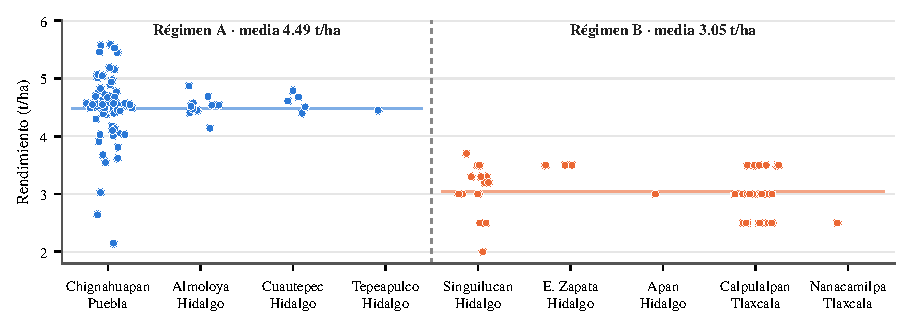
\includegraphics[width=\textwidth]{fig_regimenes}
\caption{Rendimiento de las 138 parcelas de entrenamiento por municipio. El color indica el régimen. En el régimen B
los valores se apilan en escalones de media tonelada.}\label{fig:regimenes}
\end{figure*}

\begin{table}[!t]
\caption{Rendimiento de entrenamiento por régimen}\label{tab:regimenes}
\centering\footnotesize
\begin{tabularx}{\columnwidth}{@{}lXrr@{}}
\toprule
Rég. & Municipios & Parcelas & Media (t/ha) \\
\midrule
A & Chignahuapan, Almoloya, Cuautepec de Hinojosa, Tepeapulco & 87 & 4.49 \\
B & Singuilucan, Emiliano Zapata, Apan, Calpulalpan, Nanacamilpa & 51 & 3.05 \\
\bottomrule
\end{tabularx}
\end{table}

\textbf{La separación no coincide con el estado.} El régimen se define por cómo está escrito el número, con decimales
o redondeado, y no por su valor. Hidalgo tiene municipios de los dos tipos. Almoloya, Cuautepec de Hinojosa y
Tepeapulco se parecen a Puebla, y Singuilucan, Emiliano Zapata y Apan se parecen a Tlaxcala. Agrupar por estado
mezcla dos poblaciones dentro de Hidalgo. El municipio también se conoce para las 59 parcelas de predicción, así que
el régimen se puede usar como variable.

\textbf{La causa todavía no es clara.} La diferencia puede ser real o puede deberse a la forma de medir. La
estadística oficial de 2025 va en sentido contrario a las etiquetas (Tabla~\ref{tab:siap}), lo que apunta a la forma
de medir. Por otro lado, las curvas de verdor sugieren que en el régimen B el ciclo es más corto, lo que podría
reflejar otra variedad o fecha de siembra. Para predecir, la causa importa poco, porque las 59 parcelas se califican
con etiquetas medidas igual que las de su municipio. Para interpretar los resultados sí importa, y conviene
preguntarlo a los organizadores.

\begin{table}[!t]
\caption{Media del reto y rendimiento municipal oficial de 2025, cebada de temporal~\cite{siap2026}}\label{tab:siap}
\centering\footnotesize
\begin{tabular}{@{}llrr@{}}
\toprule
Municipio & Rég. & Reto & SIAP 2025 \\
\midrule
Chignahuapan & A & 4.48 & 3.22 \\
Almoloya & A & 4.52 & 1.91 \\
Cuautepec de Hinojosa & A & 4.60 & 2.35 \\
Calpulalpan & B & 3.00 & 4.00 \\
Singuilucan & B & 3.08 & 1.88 \\
\bottomrule
\end{tabular}
\end{table}

\subsection{Valores extremos en parcelas pequeñas}
De los cinco rendimientos más altos, todos de 5.4~t/ha o más, cuatro son de parcelas de menos de 1.5 hectáreas
(Fig.~\ref{fig:area}). Con mediciones de campo se ha documentado que los productores sobreestiman el rendimiento
sobre todo en parcelas pequeñas~\cite{gourlay2019}. Si aquí pasa lo mismo, parte de esos valores es ruido de
etiqueta y no algo que el satélite pueda explicar.

\begin{figure}[!t]
\centering
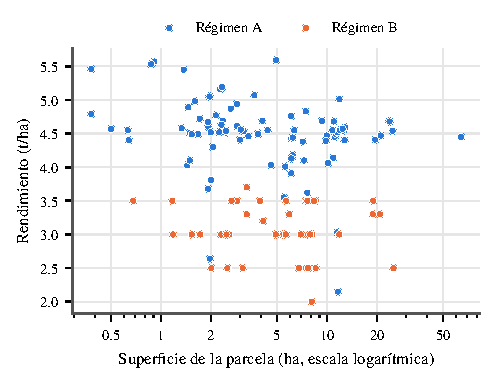
\includegraphics[width=\columnwidth]{fig_area}
\caption{Rendimiento frente al tamaño de la parcela, en escala logarítmica. Cuatro de los cinco rendimientos de
5.4~t/ha o más corresponden a parcelas de menos de 1.5 hectáreas.}\label{fig:area}
\end{figure}

\subsection{Error por redondeo}
Redondear a la media tonelada más cercana agrega por sí solo un error típico de unos 0.14~t/ha, si el valor real
puede caer en cualquier punto del escalón. En el régimen B ningún modelo podría bajar de ese error, aunque fuera
perfecto.

\subsection{La lluvia de 2025}
A nivel nacional, 2025 fue el año más lluvioso desde 1941. En la zona de las parcelas el total de junio a octubre fue
parecido al de 2024, y lo que cambió fue el momento de la lluvia (Fig.~\ref{fig:lluvia} y Tabla~\ref{tab:lluvia}).
\begin{enumerate}
  \item \textbf{Mayo y junio fueron muy lluviosos}, con el doble de lluvia que cualquiera de los tres años
        anteriores. Eso favorece sembrar a tiempo, pero puede encharcar las parcelas recién sembradas.
  \item \textbf{Julio y agosto fueron normales}, sin exceso durante el llenado de grano.
  \item \textbf{Septiembre y octubre volvieron a ser lluviosos}, en la madurez y la cosecha. En esa etapa la lluvia
        puede tumbar el cultivo, lo que se conoce como \emph{acame}, o retrasar la cosecha.
  \item \textbf{La temperatura máxima fue más fresca} que en 2023 y 2024, lo que suele favorecer el llenado del
        grano.
\end{enumerate}
Esto sugiere que los efectos del exceso de agua fueron de parcela, en zonas bajas o en parcelas cosechadas tarde, y
no de zona. El clima mensual de 5 kilómetros difícilmente los detecta.

\begin{figure}[!t]
\centering
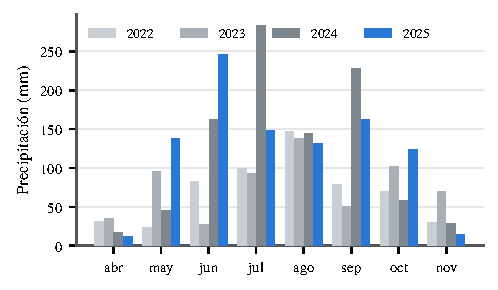
\includegraphics[width=\columnwidth]{fig_lluvia}
\caption{Precipitación mensual promedio sobre las 197 parcelas, de abril a noviembre~\cite{funk2015}.}\label{fig:lluvia}
\end{figure}

\begin{table}[!t]
\caption{Lluvia por etapa y temperatura máxima, promedio sobre las parcelas}\label{tab:lluvia}
\centering\footnotesize
\begin{tabular}{@{}lrrrr@{}}
\toprule
 & 2022 & 2023 & 2024 & 2025 \\
\midrule
Mayo y junio (mm) & 106 & 122 & 207 & \textbf{384} \\
Julio y agosto (mm) & 246 & 231 & 427 & 281 \\
Septiembre y octubre (mm) & 148 & 154 & 287 & \textbf{286} \\
Tmax de mayo a sep. (°C) & 23.7 & 24.7 & 25.0 & 23.6 \\
\bottomrule
\end{tabular}
\end{table}

\subsection{Verificación}
La Tabla~\ref{tab:verificar} indica cómo comprobar cada observación. Si los números de quien las reproduce coinciden,
la observación pasa a ser un hecho.

\begin{table}[!t]
\caption{Observaciones preliminares y cómo comprobarlas}\label{tab:verificar}
\centering\footnotesize
\begin{tabularx}{\columnwidth}{@{}>{\raggedright\arraybackslash}p{3.3cm}X@{}}
\toprule
Observación & Cómo comprobarla \\
\midrule
Dos regímenes de medición por municipio & Contar por municipio los rendimientos con dos decimales y calcular la
  media de cada grupo \\
El régimen separa mejor que el estado & Comparar la varianza explicada por cada agrupación \\
Valores extremos en parcelas pequeñas & Graficar rendimiento contra área y revisar las cinco parcelas más altas \\
Lluvia de 2025 concentrada en siembra y cosecha & Extraer CHIRPS por parcela y sumar por bimestre y año \\
Más observaciones limpias en 2025 & Contar por año las fechas con nubosidad baja entre mayo y octubre \\
Planet cubre todo 2025 & Convertir las fechas con formato día, mes y año y revisar el rango \\
Ciclo más corto en el régimen B & Estimar inicio y fin del verdor por parcela y comparar entre regímenes \\
\bottomrule
\end{tabularx}
\end{table}

\section{Hipótesis}\label{sec:hipotesis}
A partir de la revisión planteamos cinco hipótesis, ordenadas de la más probable a la más incierta. Para cada una
indicamos cómo comprobarla y qué haríamos con el resultado.

\textbf{H1. El régimen de medición explica buena parte del rendimiento.} Usar el régimen como variable base debería
mejorar la predicción frente a usar el estado. Para comprobarlo comparamos, con validación cruzada, un modelo que
predice la media de cada régimen contra uno que predice la media de cada estado. Si se confirma, el régimen será el
punto de partida de todos los modelos y reportaremos el error por régimen.

\textbf{H2. Parte del error es ruido de etiqueta.} El redondeo del régimen B y los valores extremos de las parcelas
pequeñas serían errores de medición que el modelo no debe tratar de reproducir. Para comprobarlo entrenamos dando
menos peso a los valores extremos o más peso a las parcelas grandes, y vemos si baja el error. Si no baja, tratamos a
todas las parcelas por igual.

\textbf{H3. El satélite aporta información dentro de cada régimen.} Dentro de un mismo régimen, las curvas de verdor
deberían distinguir las parcelas que rindieron más de las que rindieron menos. Las variables más prometedoras son el
ciclo alineado a la floración de cada parcela, el NDRE, el historial de 2022 a 2024, los índices de labranza antes de
la siembra y la uniformidad del cultivo dentro de la parcela. Para comprobarlo agregamos estas variables al régimen y
aplicamos la prueba de permutación. Si se confirma, es el bloque donde más conviene invertir tiempo.

\textbf{H4. Las parcelas atípicas tienen una causa visible.} Algunas parcelas con un rendimiento muy distinto al de su
grupo pudieron sufrir acame o una cosecha tardía por la lluvia de septiembre y octubre. El radar de Sentinel-1
atraviesa las nubes y su señal cambia cuando el cultivo se tumba~\cite{chauhan2020}. Para comprobarlo revisamos las
curvas de las parcelas atípicas y probamos variables de radar. Si no aparece una causa, esas parcelas se tratan como
ruido, como en H2.

\textbf{H5. El clima importa a escala de parcela, no de zona.} En un año sin falta de agua, la lluvia mensual de
5 kilómetros debería distinguir poco entre parcelas. Lo que sí podría importar es la lluvia en las semanas previas a
la floración de cada parcela. Para comprobarlo necesitamos lluvia diaria, medida en la ventana de cada parcela, y
la prueba de permutación. Si no se confirma, el clima queda sólo como descripción de la zona.

\section{Supuestos que cambian}\label{sec:supuestos}
Antes de revisar los datos, el equipo hizo una revisión de literatura y de estadística oficial. Algunos supuestos de
esa revisión no coinciden con lo que muestran los archivos (Tabla~\ref{tab:supuestos}).

\begin{table*}[!t]
\caption{Supuestos iniciales y lo que muestran los archivos}\label{tab:supuestos}
\centering\footnotesize
\begin{tabularx}{\textwidth}{@{}>{\raggedright\arraybackslash}p{4.6cm}>{\raggedright\arraybackslash}X>{\raggedright\arraybackslash}p{5.2cm}@{}}
\toprule
Supuesto inicial & Lo que muestran los archivos & Consecuencia \\
\midrule
Rendimiento esperado de 1.5 a 3.5~t/ha, según promedios estatales & La media es 3.96~t/ha y el rango va de 2.0 a 5.6 &
  Las parcelas no representan el promedio de su municipio \\
Un promedio municipal oficial serviría como referencia & El SIAP de 2025 va en sentido contrario a las etiquetas &
  El SIAP sirve sólo como contexto \\
Planet no trae información de borde rojo & Su LAI se calcula con el borde rojo y de él se recupera el NDRE &
  Hay NDRE sin datos externos \\
Planet cubre sólo parte de 2025 & Cubre de enero a diciembre & Se pueden medir la senescencia y la cosecha \\
Topografía de 15 metros & Es de 120 metros & El relieve fino requiere otra fuente \\
2024 fue un año seco & En la zona, 2024 llovió tanto como 2025 & Comparar 2025 con años previos no da anomalías extremas \\
Mucha nubosidad en la temporada de 2025 & 2025 tuvo más observaciones limpias que los años previos &
  Reconstruir las series es un problema moderado \\
La validación cruzada debe separar por zonas & La división oficial se hizo al azar & La validación cruzada debe separar al azar \\
Se puede medir el clima alrededor de la floración & El clima entregado es mensual & Hace falta clima diario \\
El redondeo de etiquetas depende del estado & Depende del municipio, y Hidalgo tiene de los dos tipos &
  El régimen reemplaza al estado como agrupación \\
\bottomrule
\end{tabularx}
\end{table*}

\section{Datos públicos}\label{sec:externos}
Las bases permiten agregar información pública. Con ella se podrían buscar dos cosas, más rendimientos para entrenar
o más información sobre las mismas parcelas.

\textbf{Más rendimientos.} No encontramos ningún conjunto público con rendimiento de cebada por parcela en la zona
(Tabla~\ref{tab:externos}). Los 138 rendimientos entregados son todo lo que hay a esa escala. Dentro del propio
conjunto, Sentinel-2 y Landsat cubren de 2022 a 2024 las mismas 197 parcelas. No traen rendimiento, pero muestran
cómo se comporta cada parcela año con año, y eso se puede usar como variable.

\begin{table}[!t]
\caption{Fuentes revisadas como posibles rendimientos}\label{tab:externos}
\centering\footnotesize
\begin{tabularx}{\columnwidth}{@{}>{\raggedright\arraybackslash}p{2.4cm}X@{}}
\toprule
Fuente & Motivo por el que no sirve \\
\midrule
SIAP, producción municipal~\cite{siap2026} & Es un promedio por municipio y va en sentido contrario a las etiquetas \\
Ensayos de variedades del CIMMYT en Valles Altos & Son parcelas experimentales de otros años y en parte con riego \\
Bitácoras de productores MasAgro & No se publican a nivel de parcela \\
\bottomrule
\end{tabularx}
\end{table}

\textbf{Más información sobre las parcelas.} Ordenamos las fuentes según lo que esperamos que aporten.
\begin{enumerate}
  \item Radar de Sentinel-1, que atraviesa las nubes y puede detectar acame y fecha de cosecha~\cite{chauhan2020}.
  \item Lluvia y temperatura diarias, para medir lo que pasó cerca de la floración de cada parcela.
  \item Bandas originales de Sentinel-2, con máscara de nubes por píxel y sin los bordes de cada parcela, que en las
        parcelas pequeñas pesan mucho.
  \item Propiedades del suelo y un modelo de elevación más fino.
  \item Representaciones anuales de imágenes satelitales publicadas por Google, de 2017 a 2024, como resumen del
        historial de cada sitio.
\end{enumerate}

\section{Regla de decisión}\label{sec:decision}
Con pocas parcelas, una idea puede parecer mejor sólo por azar (Sección~\ref{sec:problema}). Por eso fijamos la
regla antes de probar. Una idea se acepta sólo si cumple dos condiciones.
\begin{enumerate}
  \item \textbf{Le gana a la mejor versión anterior} en al menos 7 de cada 10 particiones de la validación cruzada,
        usando siempre las mismas particiones.
  \item \textbf{Pasa la prueba de permutación}, es decir, el modelo empeora cuando se revuelven sus variables nuevas.
\end{enumerate}
Las ideas que no cumplan la regla se registran como probadas y descartadas, porque también son un resultado.

\textbf{Orden de las pruebas.} Seguimos el orden de las hipótesis (Tabla~\ref{tab:orden}). La elección del algoritmo
y la combinación de modelos quedan al final, porque suelen dar las mejoras más pequeñas.

\begin{table}[!t]
\caption{Orden propuesto de las pruebas}\label{tab:orden}
\centering\footnotesize
\begin{tabularx}{\columnwidth}{@{}rX>{\raggedright\arraybackslash}p{2.1cm}@{}}
\toprule
Paso & Prueba & Mejora esperada \\
\midrule
0 & Fijar las particiones de la validación cruzada y la regla de decisión & Requisito \\
1 & Régimen como variable base (H1) & Grande \\
2 & Variables satelitales dentro de cada régimen (H3) & Pequeña a media \\
3 & Causa de las parcelas atípicas (H4) & Incierta, grande si aparece \\
4 & Entrenamiento tolerante al ruido (H2) & Pequeña \\
5 & Clima diario por parcela (H5) & Incierta \\
6 & Elección del algoritmo y combinación de modelos & Al final \\
\bottomrule
\end{tabularx}
\end{table}

\section{Conclusiones}\label{sec:conclusiones}

\begin{itemize}
  \item El reto es de interpolación. Hay que estimar el rendimiento de 59 parcelas a partir de 138 vecinas del mismo
        año, y la división entre ambos conjuntos se hizo al azar.
  \item Las imágenes satelitales son abundantes y cubren todo 2025. Lo escaso son los rendimientos, y no existe una
        fuente pública que los complemente.
  \item Los rendimientos parecen venir de dos formas de medir, separadas por municipio y no por estado. Si se
        confirma, esa variable explicará buena parte de las diferencias entre parcelas.
  \item Parte del error probablemente es ruido de etiqueta, sobre todo en el régimen redondeado y en las parcelas
        pequeñas, y ese ruido pone un piso a lo que se puede lograr.
  \item En 2025 importó más cuándo llovió que cuánto, y sus efectos fueron de parcela y no de zona.
  \item Con 138 parcelas, las mejoras pequeñas pueden ser azar. Toda idea pasa por la misma regla de decisión.
  \item Lo observado hasta ahora es preliminar y debe comprobarse de forma independiente antes de apoyar una
        decisión.
\end{itemize}


\begin{thebibliography}{99}
\bibitem{bases} FIRA, \emph{Reto AgroCebada 2026. Bases de participación y descripción del conjunto de datos},
  2026.
\bibitem{funk2015} C. Funk \emph{et al.}, ``The climate hazards infrared precipitation with stations, a new
  environmental record for monitoring extremes,'' \emph{Scientific Data}, vol.~2, art.~150066, 2015,
  doi 10.1038/sdata.2015.66.
\bibitem{chirts} Climate Hazards Center, ``CHIRTS-ERA5 data repository,'' University of California, Santa
  Barbara, 2025, doi 10.15780/G2F08J.
\bibitem{inegi} INEGI, \emph{Continuo de Elevaciones Mexicano 4.0}. Aguascalientes, México, INEGI, 2025.
\bibitem{siap2026} SIAP, ``Producción agrícola municipal, cierre 2025,'' Datos abiertos, 2026. Consultado el 4 de
  octubre de 2026. Disponible en \url{https://nube.agricultura.gob.mx/datosAbiertos/Agricola.php}
\bibitem{arisnabarreta2008} S. Arisnabarreta y D. J. Miralles, ``Critical period for grain number establishment of
  near isogenic lines of two- and six-rowed barley,'' \emph{Field Crops Research}, vol.~107, no.~3, pp.~196-202,
  2008.
\bibitem{desanceledonio2014} R. P. de San Celedonio, L. G. Abeledo y D. J. Miralles, ``Identifying the critical
  period for waterlogging on yield and its components in wheat and barley,'' \emph{Plant and Soil}, vol.~378,
  pp.~265-277, 2014.
\bibitem{wadoux2021} A. M. J.-C. Wadoux, G. B. M. Heuvelink, S. de Bruin y D. J. Brus, ``Spatial cross-validation
  is not the right way to evaluate map accuracy,'' \emph{Ecological Modelling}, vol.~457, art.~109692, 2021.
\bibitem{ojala2010} M. Ojala y G. C. Garriga, ``Permutation tests for studying classifier performance,''
  \emph{Journal of Machine Learning Research}, vol.~11, pp.~1833-1863, 2010.
\bibitem{varoquaux2018} G. Varoquaux, ``Cross-validation failure. Small sample sizes lead to large error bars,''
  \emph{NeuroImage}, vol.~180, pp.~68-77, 2018.
\bibitem{cawley2010} G. C. Cawley y N. L. C. Talbot, ``On over-fitting in model selection and subsequent selection
  bias in performance evaluation,'' \emph{Journal of Machine Learning Research}, vol.~11, pp.~2079-2107, 2010.
\bibitem{gourlay2019} S. Gourlay, T. Kilic y D. B. Lobell, ``A new spin on an old debate. Errors in farmer-reported
  production and their implications for inverse scale-productivity relationship in Uganda,'' \emph{Journal of
  Development Economics}, vol.~141, 2019.
\bibitem{chauhan2020} S. Chauhan, R. Darvishzadeh, Y. Lu, M. Boschetti y A. Nelson, ``Understanding wheat lodging
  using multi-temporal Sentinel-1 and Sentinel-2 data,'' \emph{Remote Sensing}, vol.~12, no.~23, art.~3885, 2020.
\end{thebibliography}

\end{document}
